\icode{O-MM-SU-261010}
\lkf{物理模型}

\noindent 质量为\(M\)木板\(B\)静止在光滑的地面上，质量为\(m\)滑块\(A\)以初速度\(v_0\)滑上木板\(B\)，滑块\(A\)与木板\(B\)的摩擦力系数为\(\mu\)。经过一段时间\(t\)后，滑块没有滑下木板，滑块\(A\)和木板\(B\)的速度分别为\(v_1\)、\(v_2(v_1 \geq v_2)\)，滑块\(A\)和木板\(B\)的位移分别为\(x_1\)、\(x_2\)，如图所示

\begin{figure}[htbp]
	\centering
	\begin{tikzpicture}[>=latex,scale=.8,font=\scriptsize]
		\draw (0,0) rectangle(2,.5);
		\draw (0,.5) rectangle(.5,1);
		\draw[teal] (5,-2) rectangle(7,-1.5);
		\draw[teal] (6,-1.5) rectangle(6.5,-1);
		\draw[dashed](0,1.5)--(0,-2);
		\draw[dashed](5,-.5)--(5,-2);
		\draw[dashed](6,-1)--(6,1.5);
		\draw[->,blue] (.5,.8)--(1.5,.8)node[right]{\(v_0\)};
		\draw[->,cyan] (6.5,-1.25)--(7.3,-1.25)node[right]{\(v_1\)};
		\draw[->,cyan] (7,-1.75)--(7.5,-1.75)node[right]{\(v_2\)};
		\draw[->,red] (0,.75)--(-1,.75)node[left]{\(f\)};
		\draw[->,red] (2,.25)--(3,.25)node[right]{\(f^\prime\)};
		\draw[->,orange] (0,-1.7)--node[fill=white]{\(x_2\)}(5,-1.7);
		\draw[->,orange] (0,1.3)--node[fill=white]{\(x_1\)}(6,1.3);
		\draw[->,orange] (5,-.8)--node[below]{\(x_\text{相}\)}(6,-.8);
		\draw[thick] (-.5,0)--(7.5,0);
		\foreach \x in {-.5,-.3,...,7.2} 
			\draw[gray] (\x,-.2)--++(.2,.2);
		\draw[gray] (-.5,-2)--(7.5,-2);
		\foreach \x in {-.5,-.3,...,7.2} 
			\draw[gray!70] (\x,-2.2)--++(.2,.2);
		\node at(1,.25){\(B\)};
		\node at(.2,.75){\(A\)};
		\node[teal] at(6,-1.75){\(B\)};
		\node[teal] at(6.2,-1.25){\(A\)};
	\end{tikzpicture}
\end{figure}
静摩擦力与滑动摩擦力

\lkf{静摩擦力：}一个物体在另一个物体表面上具有{\kaishu\color{red} 相对运动趋势}时，但并没有发生相对运动时，所受到的阻碍物体相对运动趋势的力叫静摩擦力。
\begin{figure}[htbp]
	\centering
	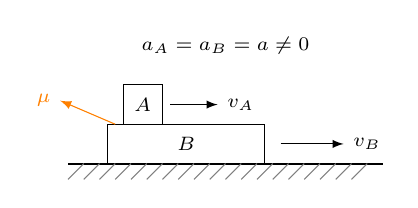
\begin{tikzpicture}[>=latex,font=\scriptsize]
		\draw (0,0) rectangle(2,.5);
		\draw (.2,.5) rectangle(.7,1);
		\draw[->,orange] (.1,.5)--(-.6,.8)node[left]{\(\mu\)};
		\draw[thick] (-.5,0)--(3.5,0);
		\foreach \x in {-.5,-.3,...,3.2} 
			\draw[gray] (\x,-.2)--++(.2,.2);
		\node at(1,.25){\(B\)};
		\node at(.45,.75){\(A\)};
		\draw[->] (.8,.75)--(1.4,.75)node[right]{\(v_A\)};
		\draw[->] (2.2,.25)--(3,.25)node[right]{\(v_B\)};
		\node at(1.5,1.5){\(a_A = a_B = a\ne 0\)};
	\end{tikzpicture}
	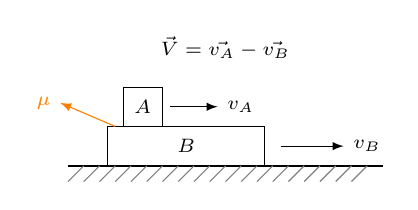
\begin{tikzpicture}[>=latex,font=\scriptsize]
		\draw (0,0) rectangle(2,.5);
		\draw (.2,.5) rectangle(.7,1);
		\draw[->,orange] (.1,.5)--(-.6,.8)node[left]{\(\mu\)};
		\draw[thick] (-.5,0)--(3.5,0);
		\foreach \x in {-.5,-.3,...,3.2} 
			\draw[gray] (\x,-.2)--++(.2,.2);
		\node at(1,.25){\(B\)};
		\node at(.45,.75){\(A\)};
		\draw[->] (.8,.75)--(1.4,.75)node[right]{\(v_A\)};
		\draw[->] (2.2,.25)--(3,.25)node[right]{\(v_B\)};
		\node at(1.5,1.5){\(\vec{V}=\vec{v_A}-\vec{v_B}\)};
	\end{tikzpicture}
\end{figure}
	
{\fangsong 在板块模型这这里，如果物体\(A\)在木板\(B\)上所受的力是静摩擦，那么物体\(A\)和木板\(B\)一定没有相对运动，即相对速度为\(0\)，即\(v_A = v_B\)。而且经分析可知\(AB\)具有相同的加速度\(a\)\((a\ne0)\)，\(A\)受到的摩擦力大小为\(f_{\text{静}} = m_A a\)，方向与加速度的方向相同。若\(AB\) 以相同的速度做匀速直线运动，\(AB\)之间没有摩擦力。}

\lkf{滑动摩擦力：}当一个物体在另一物体表面滑动时，会受到时另一个物体阻碍它物体滑动的力，这种力称为滑动摩擦力，方向与相对运动的方向相反。

{\fangsong 如下图所示，\(A\)对\(B\)的相对速度记为\(\vec{V}(V\ne0)\)，则\(A\)受到的滑动摩擦力大小为
	\[f_\text{滑}=\mu N=\mu m_A g\]
滑动摩擦力的方向与相对速度\(\vec{V}\)的方向相反。式中\(N\)为正压力。
}

\begin{figure}[htbp]
	\begin{minipage}{0.49\textwidth}
		\centering
		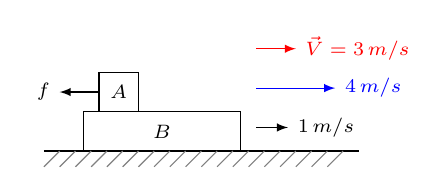
\begin{tikzpicture}[>=latex,font=\scriptsize]
			\draw (0,0) rectangle(2,.5);
			\draw (.2,.5) rectangle(.7,1);
			\draw[thick] (-.5,0)--(3.5,0);
			\foreach \x in {-.5,-.3,...,3.2}
				\draw[gray] (\x,-.2)--++(.2,.2);
			\node at(1,.25){\(B\)};
			\node at(.45,.75){\(A\)};
			\draw[->,blue] (2.2,.8)--(3.2,.8)node[right]{\(4\,m/s\)};
			\draw[->] (2.2,.3)--(2.6,.3)node[right]{\(1\,m/s\)};
			\draw[->,red] (2.2,1.3)--(2.7,1.3)node[right]{\(\vec{V} = 3\,m/s\)};
			\draw[->] (.2,.75)--(-.3,.75)node[left]{\(f\)};
		\end{tikzpicture}
	\end{minipage}
	\begin{minipage}{0.49\textwidth}
		\centering
		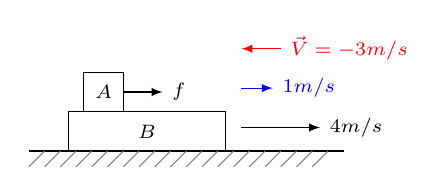
\begin{tikzpicture}[>=latex,font=\scriptsize]
			\draw (0,0) rectangle(2,.5);
			\draw (.2,.5) rectangle(.7,1);
			\draw[thick] (-.5,0)--(3.5,0);
			\foreach \x in {-.5,-.3,...,3.2}
				\draw[gray] (\x,-.2)--++(.2,.2);
			\node at(1,.25){\(B\)};
			\node at(.45,.75){\(A\)};
			\draw[->,blue] (2.2,.8)--(2.6,.8)node[right]{\(1m/s\)};
			\draw[->] (2.2,.3)--(3.2,.3)node[right]{\(4m/s\)};
			\draw[->,red] (2.7,1.3)node[right]{\(\vec{V} = -3m/s\)}--(2.2,1.3);
			\draw[->] (.7,.75)--(1.2,.75)node[right]{\(f\)};
		\end{tikzpicture}
	\end{minipage}
\end{figure}
摩擦力的冲量与动量守恒
	
我们依用上述物理模型分析冲量与动量的关系。将滑块\(A\)与木板\(B\)视作一个系统，它们之间的滑动摩擦力就是内力，系统动量守恒。

{\fangsong 以水平向右为正方向，滑块\(A\)受到滑动摩擦力\(f\)的冲量
\[I_f =- ft =-\mu mgt = mv_1 - mv_0 =\Delta p_A\]
木板\(B\)受到滑动摩擦力\(f^\prime\)的冲量
\[I_{f^\prime} =f^\prime t =\mu mgt = Mv_2 - 0 =\Delta p_B\]
由此可知滑块与木板之间摩擦力的合冲量
\[\begin{aligned}
	I_\text{合}&= I_f + I_{f^\prime}=-ft + f^\prime t= 0 \\
	\Rightarrow mv_0&= mv_1 + Mv_2\\
	\Rightarrow \Delta p_A &=-\Delta p_B
\end{aligned}\]
我们可以这样理解上面的等式，作为内力的滑动摩擦力不改变系统的总动量。换个说法，滑块\(A\)减少的动量\(\Delta p\)，通过摩擦力百分百传递给了木板\(B\)，木板\(B\)的动量增加了\(\Delta p\)，因此系统的总动量不变。
}
摩擦力做功与摩擦起热

 我们依旧沿用上面的物理模型分析摩擦力做功问题

{\fangsong 受力分析可知，滑块\(A\)受到的滑动摩擦力大小为\(f =\mu mg\)，方向水平向左，是阻力做负功
\[W_f = -fx_1 =-\mu mgx_1 = \frac{1}{2}mv_1^2 - \frac{1}{2}mv_0^2\]
木板\(B\)受到的滑动摩擦力大小为\(f^\prime=\mu mg\)，方向水平向右，是动力做正功
\[W_{f^\prime}= f^\prime x_2 =\mu mgx_2 = \frac{1}{2}Mv_2^2 - 0\]
那么滑块\(A\)与木板\(B\)之间摩擦力做的总功，即摩擦力\(f\)和\(f^\prime\)做功的算术和
\[\begin{aligned}
	W_\text{总} &= W_f + W_{f^\prime}\\
	&=- fx_1 + f^\prime x_2 =-\mu mg(x_1 - x_2) =-\mu mgx_\text{相}\\
	&=-[\frac{1}{2}mv_0^2 - (\frac{1}{2}mv_1^2 + \frac{1}{2}Mv_2^2)]\\
	&=-\Delta E_{k\text{损}}
\end{aligned}\]
经以上分析可知，我们可以认为滑块\(A\)的动能以摩擦力做功的方式传递给木板\(B\)，但是摩擦力不能百分百传递动能，滑块\(A\)的一部分动能在传递给\(B\)的过程中损失了一些，损失的这部分动能转化为内能（热量），记作\(Q\)
\[\begin{aligned}Q &= fx_\text{相}\\
	&=\frac{1}{2}mv_0^2 - (\frac{1}{2}mv_1^2 + \frac{1}{2}Mv_2^2)\\
	&=\Delta E_{k\text{损}}
\end{aligned}\]
}